% !TeX program = xelatex
\documentclass[11pt]{paper}

\usepackage{ctex}
\usepackage{fontspec}
\usepackage{setspace}
\usepackage[a4paper, margin=3cm]{geometry}

%图
\usepackage{graphicx}
\usepackage{subfig}    %% 子图包
\usepackage{float}     %% 浮动

\usepackage[colorlinks,linkcolor=black,anchorcolor=black,citecolor=black]{hyperref}
\usepackage{indentfirst} %缩进
\usepackage{amsmath}

\setmainfont{Times New Roman}

% \title{
%     实验报告 \\ 
%     西电B测 \\
%     实现2PSK 2DPSK调制解调系统
%     }
% \author{陈禹译\ \ 刘怡君\ \ 史卓一}
% \date{2023/5/11}

\begin{document}

%下方居中显示页码
\pagestyle{plain}

\begin{titlepage}
    \begin{center}
        \vspace{4mm}  %间距
        \begin{spacing}{2}%行距2
            \Huge{西安电子科技大学B测\ 实验报告 \\ \textbf{实现2PSK 2DPSK调制解调系统} }
        \end{spacing}

        \vspace{4mm}  %间距

        
\includegraphics[width=4.4in]{texture/xdlogo.png}

        \vspace{16mm}  %间距

        \Large{
            \begin{tabular}{ll}
                \vspace{2mm}  %间距
                \textbf{组号:}   & 9900                  \\
                \textbf{学生一:}  & 陈禹译 \quad 20009200485 \\
                \textbf{学生二:}  & 刘怡君 \quad 20049200450 \\
                \vspace{2mm}  %间距
                \textbf{学生三:}  & 史卓一 \quad 20009201035 \\
                \textbf{验收日期:} & 2023.5.10
            \end{tabular}
        }
    \end{center}
\end{titlepage}

\newpage
\pagenumbering{Roman}

%目录页
\vspace{10mm}
\setcounter{tocdepth}{2}%只显示到2级标题
\tableofcontents

\newpage
%正文
\pagenumbering{arabic}
\zihao{-4} %默认小四号字体

\setlength{\baselineskip}{20pt}

\section{实验目的}

利用SystemVue或Simulink实现2PSK/2DPSK调制解调系统。

\section{仿真环境}

操作系统:Windows。

仿真软件:MATLAB R2023a Simulink。

MATLAB包:Simulink 10.7,Communications Toolbox 8.0,DSP System Toolbox 9.16,Signal Processing Toolbox 9.2。

\section{系统设计}

\subsection{概览}

系统整体如图 \ref{系统整体图} ,左上为载波,左中为原信号;上半部分为2PSK,下半部分为2DPSK。
接收端的载波信号都设置了一个Gain组件,可以让载波信号反相,从而观察倒$\pi$现象。

原信号的码元速率为$9600/s$;载波频率为$5*9600*2*\pi \ rad/s$。因此每个信号都包含五个载波周期。

\begin{figure}[ht]
    \centering
    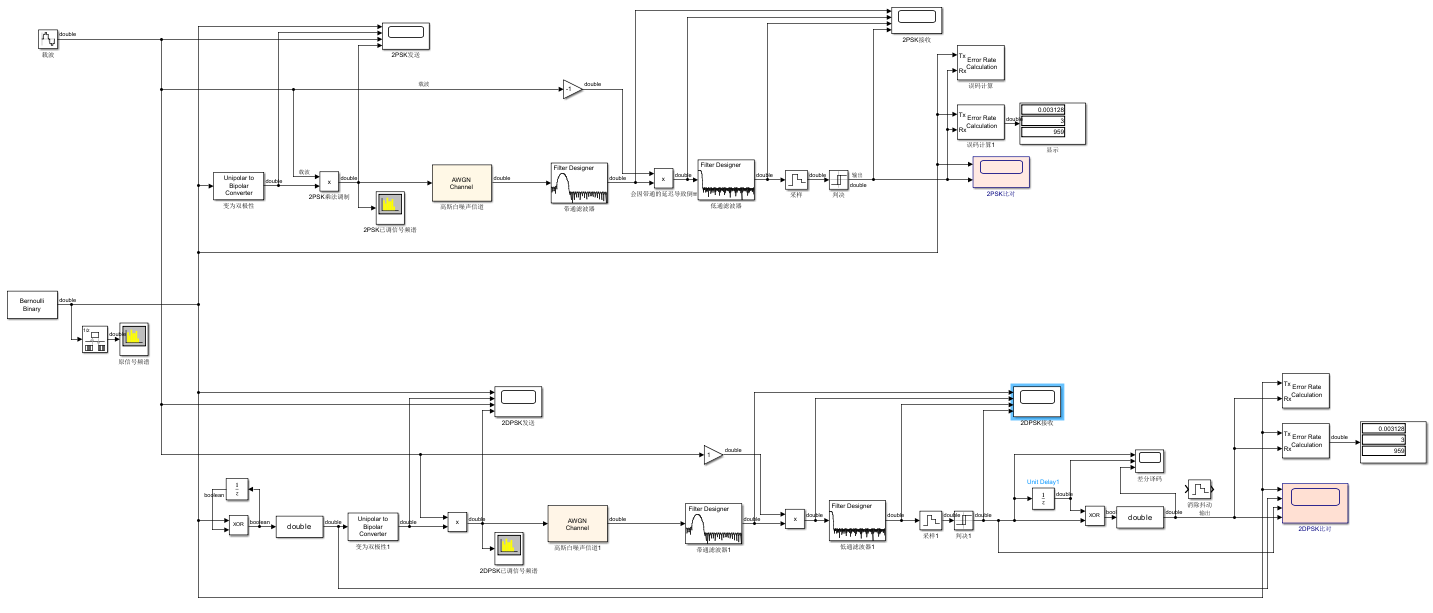
\includegraphics[width=5.9in]{texture/design/all.png}
    \caption{系统整体图}
    \label{系统整体图}
\end{figure}

\subsection{2PSK}

\subsubsection{发送}

2PSK的发送部分如图 \ref{2PSK发送部分} 。首先,将原信号变成双极性信号(从0/1变成-1/1);
然后,与载波直接相乘,即可得到已调信号:

$$
    S_{2PSK}(t)=
    \begin{cases}
        sin(\omega _{c}t)\ ,\ signal=1 \\
        -sin(\omega _{c}t)\ ,\ signal=0
    \end{cases}
$$

\begin{figure}[ht]
    \centering
    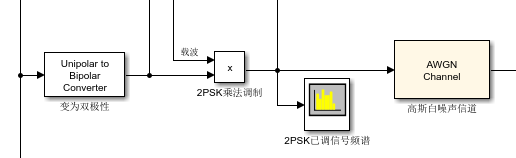
\includegraphics[width=5.9in]{texture/design/2psk1.png}
    \caption{2PSK发送部分}
    \label{2PSK发送部分}
\end{figure}

\subsubsection{接收}

解调分为过带通、乘载波、过低通、抽样判决四个部分,设计如图 \ref{2PSK接收部分} 。

\begin{figure}[ht]
    \centering
    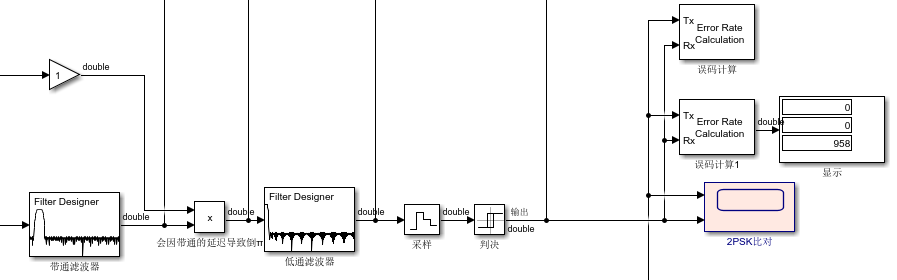
\includegraphics[width=5.9in]{texture/design/2psk2.png}
    \caption{2PSK接收部分}
    \label{2PSK接收部分}
\end{figure}

带通滤波器设计如图 \ref{带通滤波器设计},Fs符合载波信号的采样频率,也即符合原调制信号的采样频率;
而可通频率的中点为5*9600,即为载波信号的频率。

阶数自动设为50,群延迟为25sample,使得该滤波器的延迟恰为半个码元。由于每个码元对应的载波信号周期
为奇数,因此这会导致延迟了非整数周期(2.5个周期)。

\begin{figure}[ht]
    \centering
    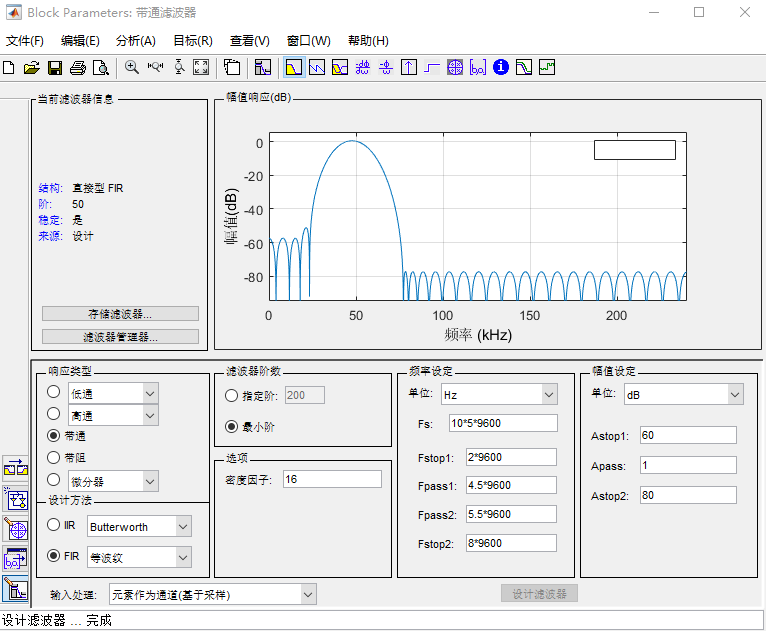
\includegraphics[width=5.9in]{texture/design/带通滤波器.png}
    \caption{带通滤波器设计}
    \label{带通滤波器设计}
\end{figure}

与载波再相乘时,因为带通滤波器延迟了2.5个周期,所以直接乘的结果会和预期相反。

原预期:
$$
    M_{2PSK}(t)=
    \begin{cases}
        sin^2(\omega _{c}t)\ ,\ signal=1 \\
        -sin^2(\omega _{c}t)\ ,\ signal=0
    \end{cases}
$$

延迟导致的现实情况:
$$
    M_{2PSK}(t)=
    \begin{cases}
        sin(\omega _{c}(t-2.5*T_{c}/2))*sin(\omega _{c}t)=-sin^2(\omega _{c}t)\ ,\ signal=1 \\
        -sin(\omega _{c}(t-2.5*T_{c}/2))*sin(\omega _{c}t)=sin^2(\omega _{c}t)\ ,\ signal=0
    \end{cases}
$$

为了修正,此乘法器的载波输入要反相(使用Gain组件,设定增益为-1)。

修正后,输出就满足了原预期:当原信号为0时,输出必为负;当原信号为1时,输出必为正。

低通滤波器设计如图 \ref{低通滤波器设计}。自动设定阶数为132,群延迟为66sample。

\begin{figure}[ht]
    \centering
    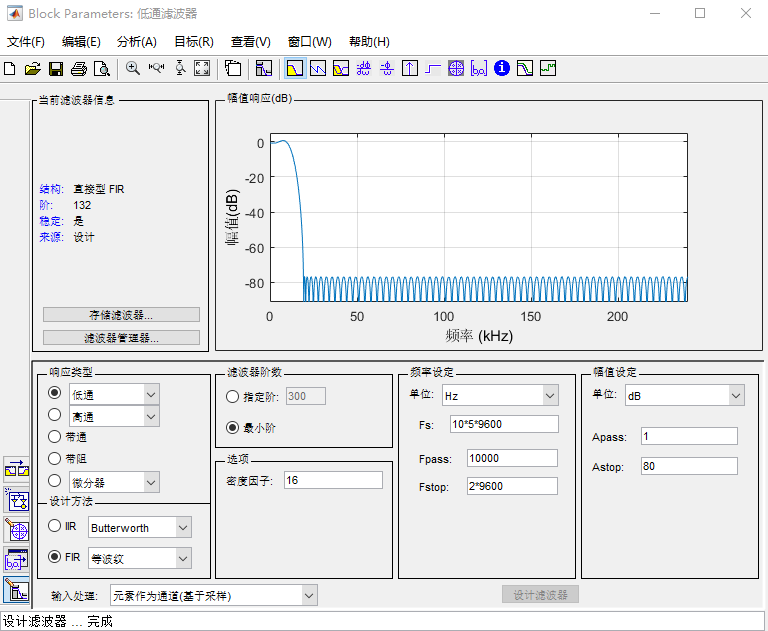
\includegraphics[width=5.9in]{texture/design/低通滤波器.png}
    \caption{低通滤波器设计}
    \label{低通滤波器设计}
\end{figure}

两个滤波器的延迟总和为$ (25+66)/50 * 100\%=182\% $倍的码元长度,略小于两倍。这使得解调结果延迟
两个码元,且采样时都避开了码元改变的时间点(零点)。

然后,使用零阶保持器对过低通的信号进行采样时间为1/9600的采样,再使用Relay进行判决,输出0和1,即为解调结果信号。

最后,输送到误码率计算器。此处设置了两个误码率计算器,一个输出到显示组件,一个输出到工作区用于绘制误码曲线。
要设置其Receive Delay属性为2sample以贴合接收信号的延迟。

\subsection{2DPSK}

\subsubsection{发送}

2DPSK的发送部分如图 \ref{2DPSK发送部分} 。相比于2PSK多了个差分编码部分,即与上一个输出进行异或后再输出(1异或等价于取非,使得输出翻转)。

\begin{figure}[ht]
    \centering
    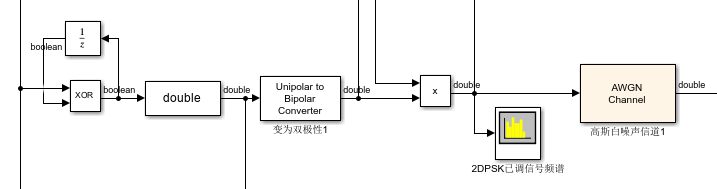
\includegraphics[width=5.9in]{texture/design/2dpsk1.png}
    \caption{2DPSK发送部分}
    \label{2DPSK发送部分}
\end{figure}

\subsubsection{接收}

2DPSK的接收部分如图 \ref{2DPSK接收部分} 。比2PSK多了个差分译码部分,即与下一个码元进行异或后再输出(与下一个码元一样则说明不翻转,为0,否则为1)。

差分译码的延迟器可能不完全准确,有较小可能在异或后在信号变化处出现抖动,此时也会报Warning提示误码率计算器的两个输入口频率不一致。在输出口加上零阶保持器能很好地解决该问题。

\begin{figure}[ht]
    \centering
    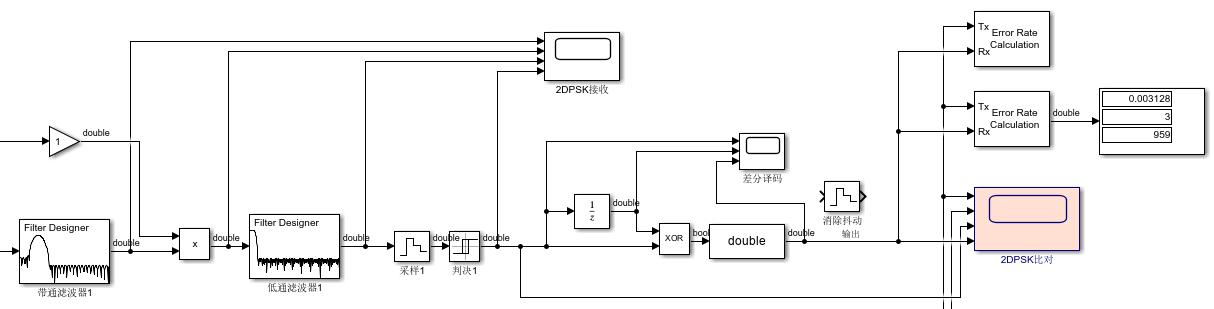
\includegraphics[width=5.9in]{texture/design/2dpsk2.png}
    \caption{2DPSK接收部分}
    \label{2DPSK接收部分}
\end{figure}

\section{仿真结果}

\subsection{频谱图}

见图\ref{原信号频谱}、图\ref{2PSK已调信号频谱}、图\ref{2DPSK已调信号频谱}。

\begin{figure}[H]
    \centering
    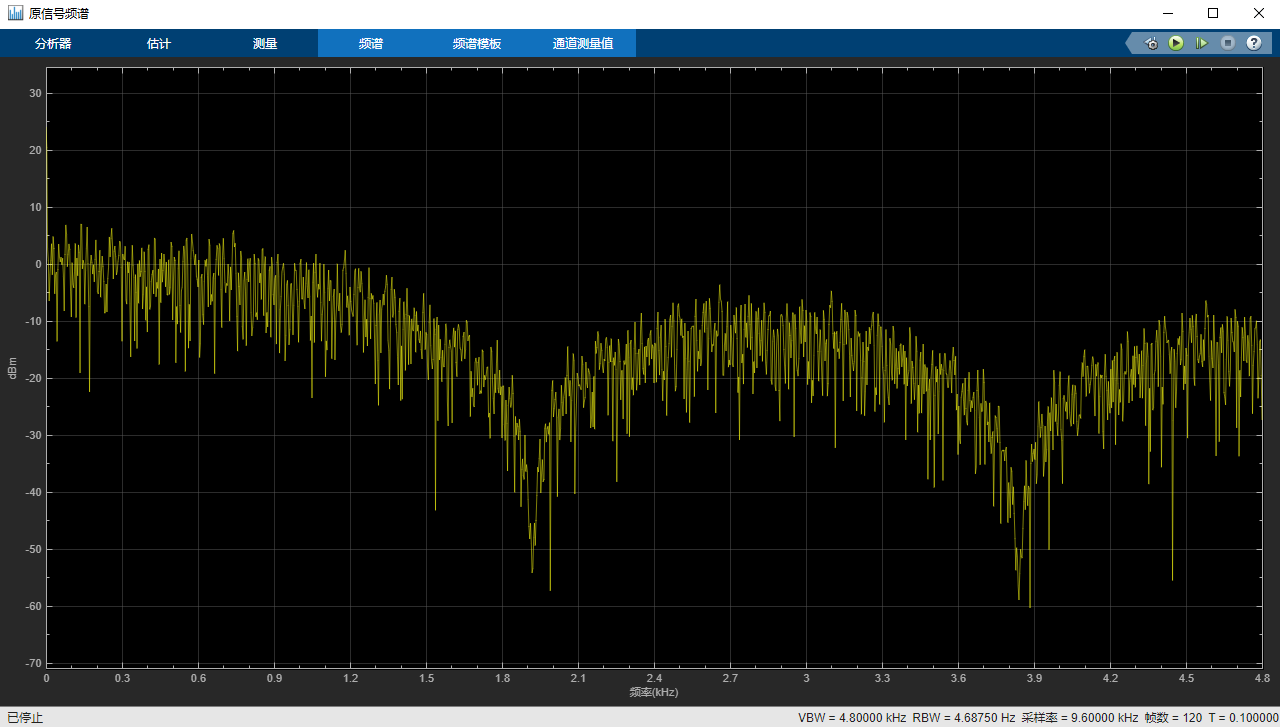
\includegraphics[width=5.9in]{texture/result/原信号频谱.png}
    \caption{原信号频谱}
    \label{原信号频谱}
\end{figure}

\begin{figure}[H]
    \centering
    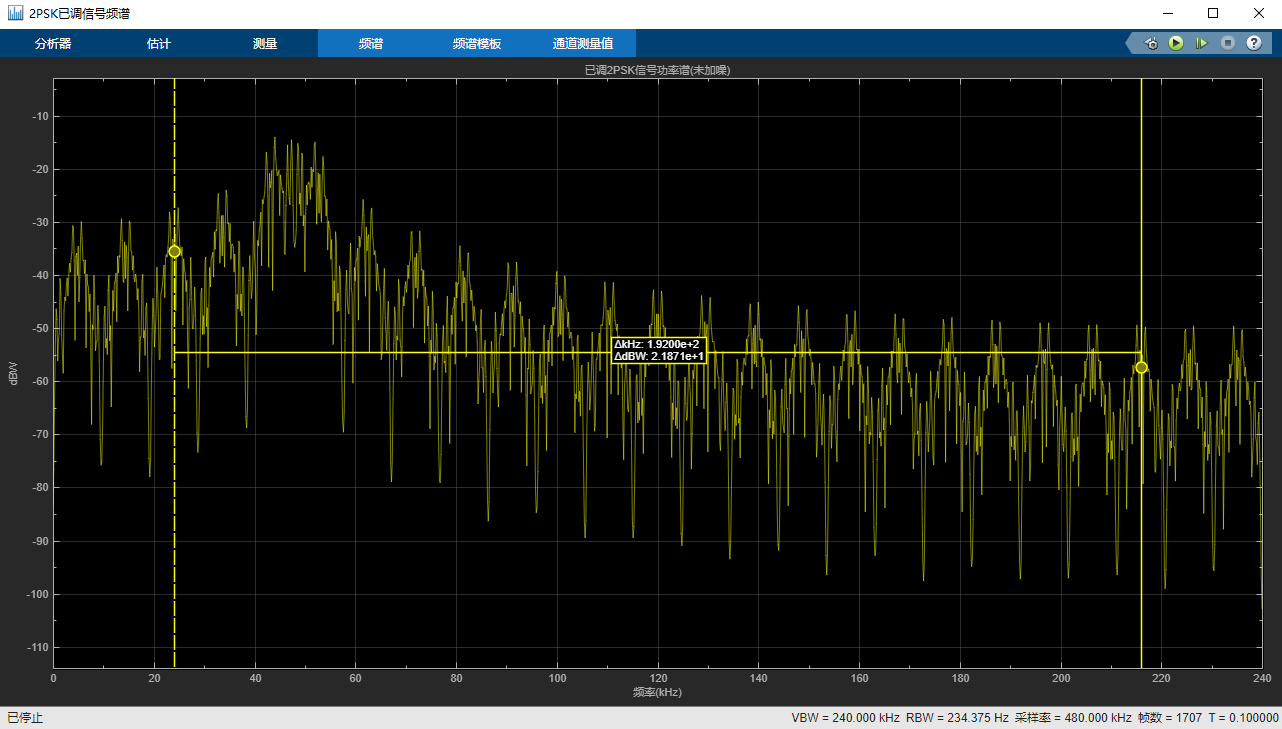
\includegraphics[width=5.9in]{texture/result/2psk频谱.png}
    \caption{2PSK已调信号频谱}
    \label{2PSK已调信号频谱}
\end{figure}

\begin{figure}[H]
    \centering
    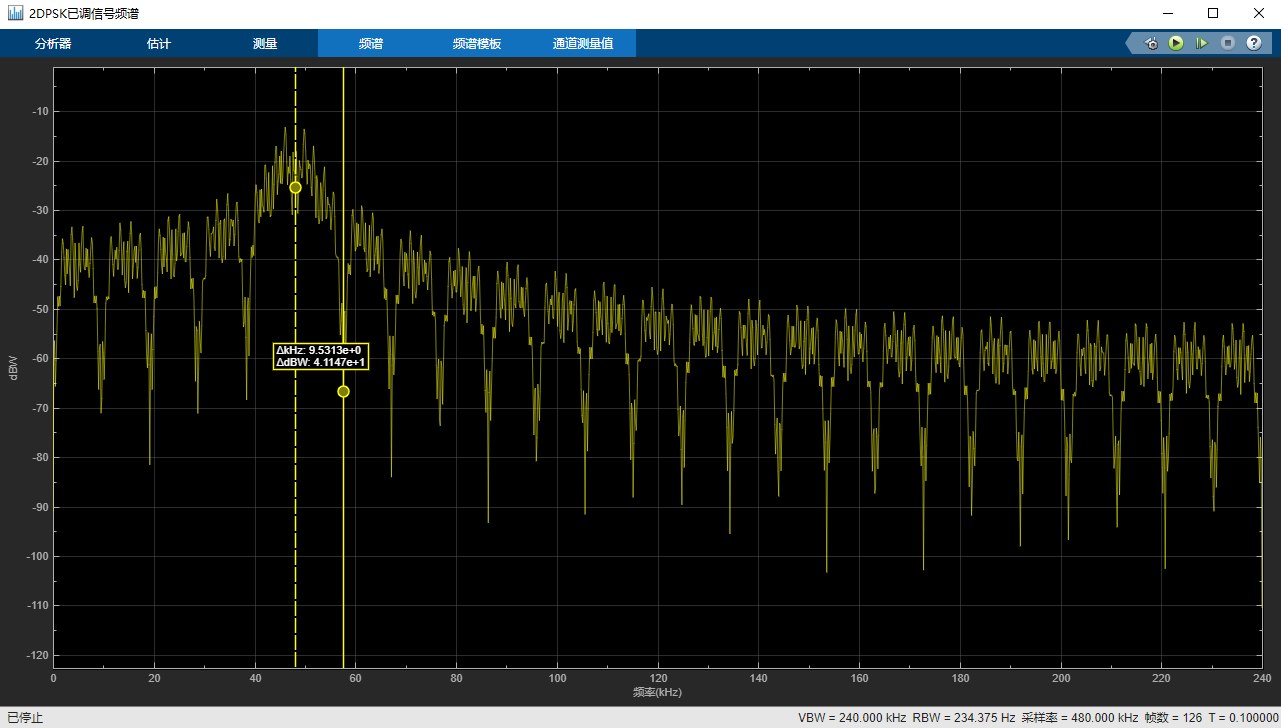
\includegraphics[width=5.9in]{texture/result/2dpsk频谱.png}
    \caption{2DPSK已调信号频谱}
    \label{2DPSK已调信号频谱}
\end{figure}

\subsection{2PSK调制解调}

见图\ref{2PSK发送}、图\ref{2PSK接收}、图\ref{2PSK比对}。

从图\ref{2PSK比对}的比对中可以看出,输出信号比原信号延迟了两个码元,是两个滤波器的延迟叠加的结果,
符合系统设计时的论证。

\begin{figure}[H]
    \centering
    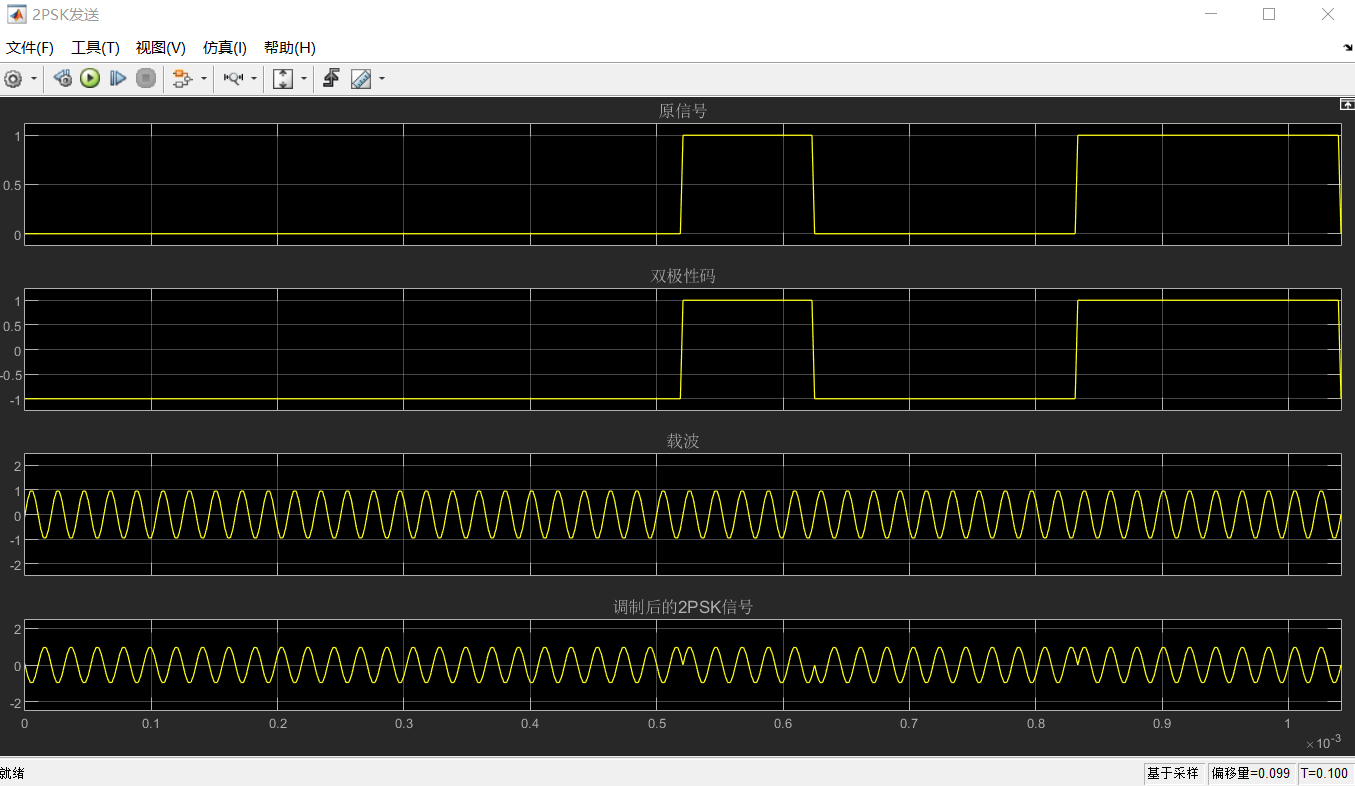
\includegraphics[width=5.9in]{texture/result/2psk发送结果.png}
    \caption{2PSK发送}
    \label{2PSK发送}
\end{figure}

\begin{figure}[H]
    \centering
    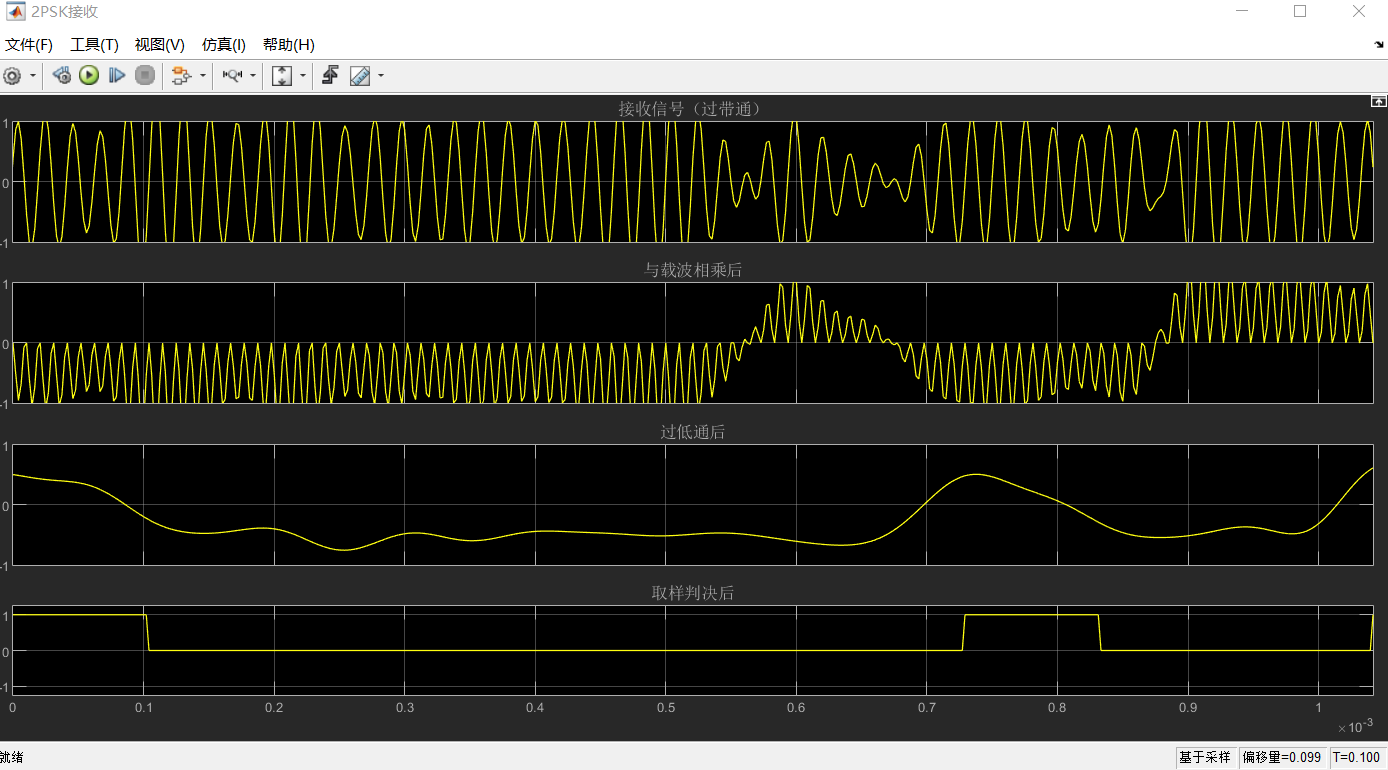
\includegraphics[width=5.9in]{texture/result/2psk接收结果.png}
    \caption{2PSK接收}
    \label{2PSK接收}
\end{figure}

\begin{figure}[H]
    \centering
    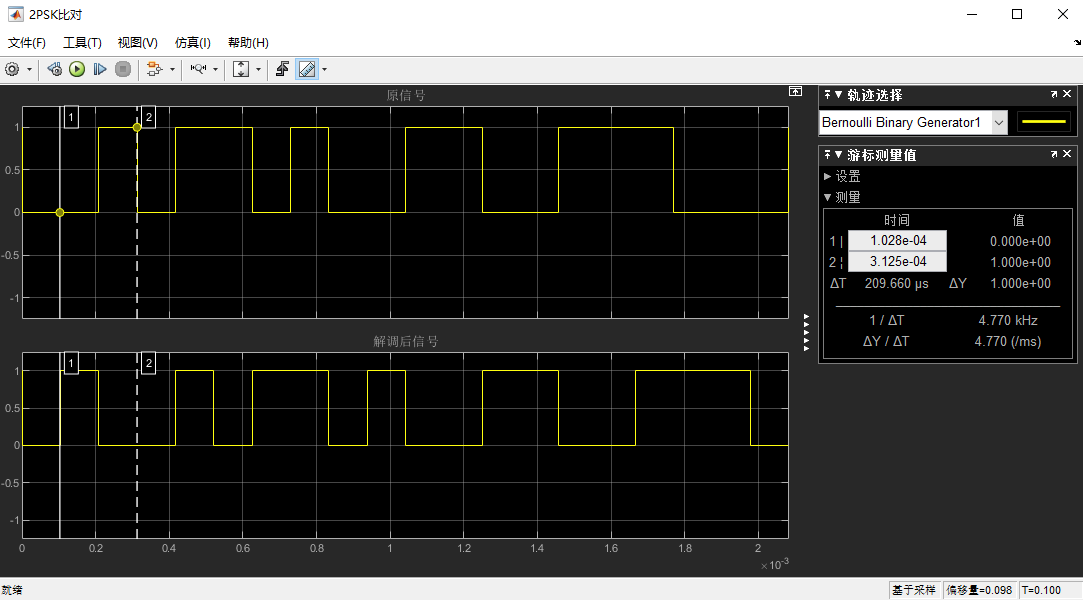
\includegraphics[width=5.9in]{texture/result/2psk比对.png}
    \caption{2PSK比对}
    \label{2PSK比对}
\end{figure}

\subsection{2DPSK调制解调}

见图\ref{2DPSK发送}、图\ref{2DPSK接收}、图\ref{2DPSK比对}。

图\ref{2PSK比对}也表明输出信号比原信号延迟了两个码元。

\begin{figure}[H]
    \centering
    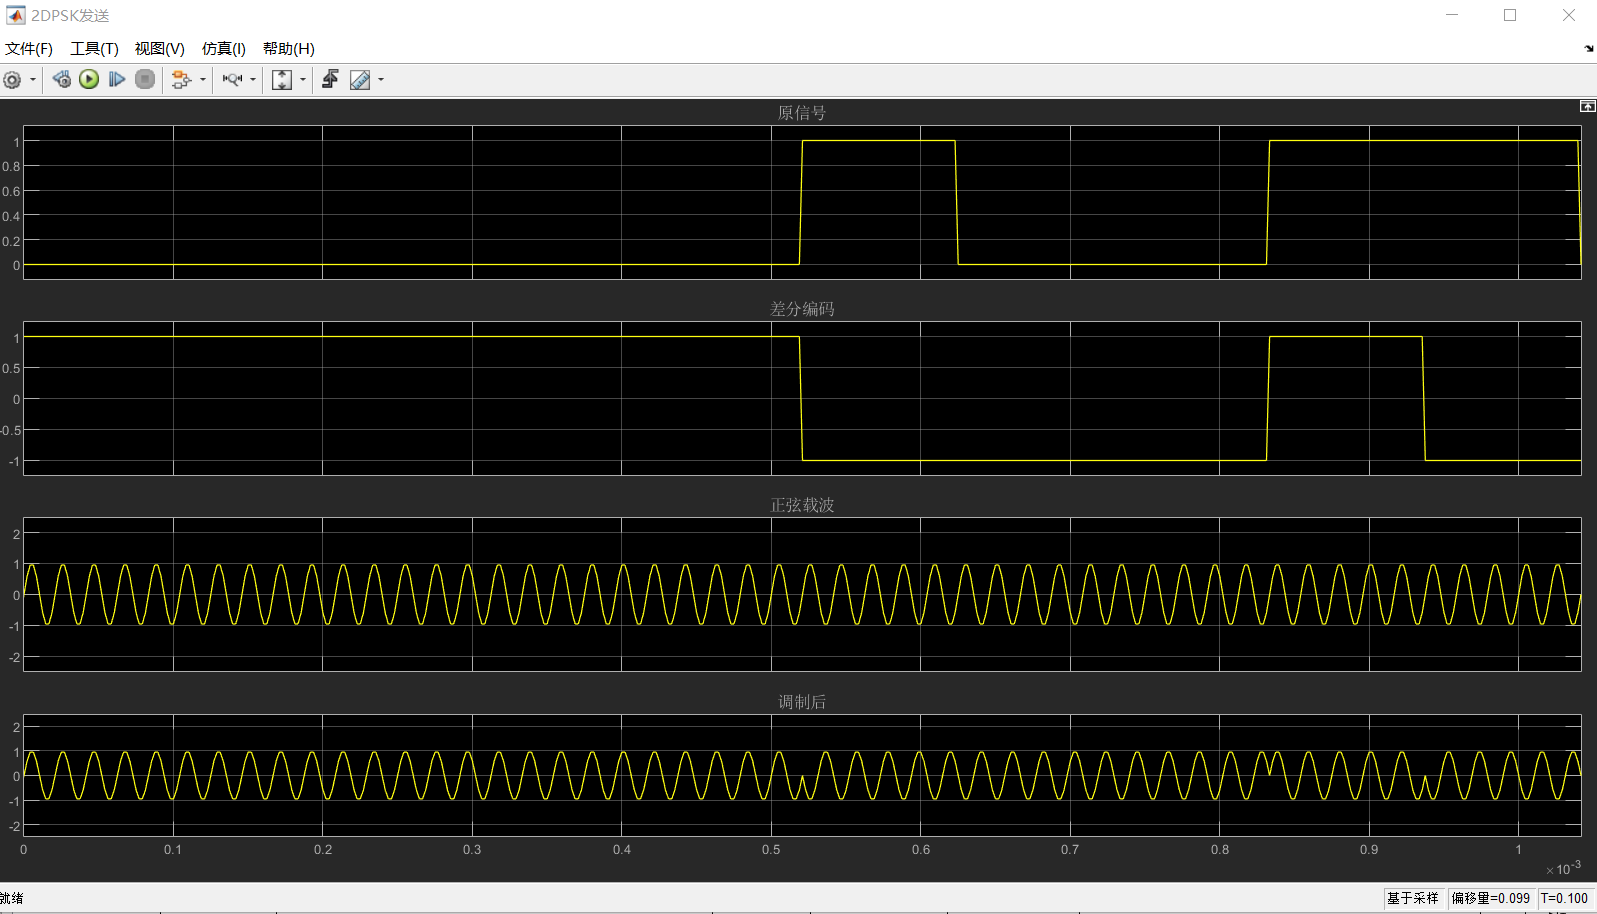
\includegraphics[width=5.9in]{texture/result/2dpsk发送结果.png}
    \caption{2DPSK发送}
    \label{2DPSK发送}
\end{figure}

\begin{figure}[H]
    \centering
    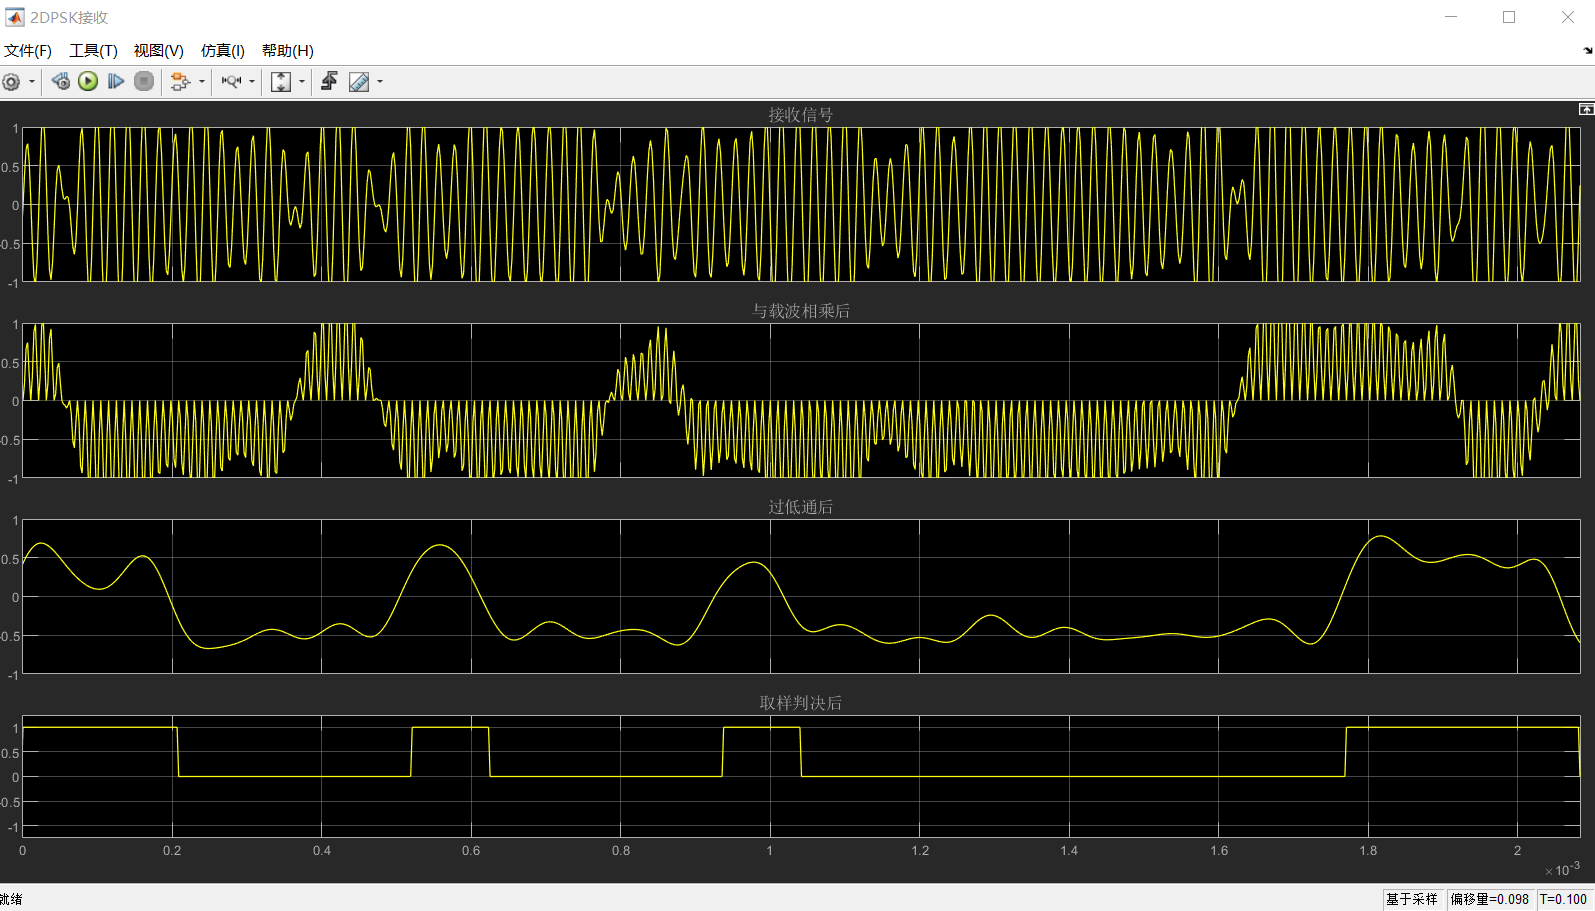
\includegraphics[width=5.9in]{texture/result/2dpsk接收结果.png}
    \caption{2DPSK接收}
    \label{2DPSK接收}
\end{figure}

\begin{figure}[H]
    \centering
    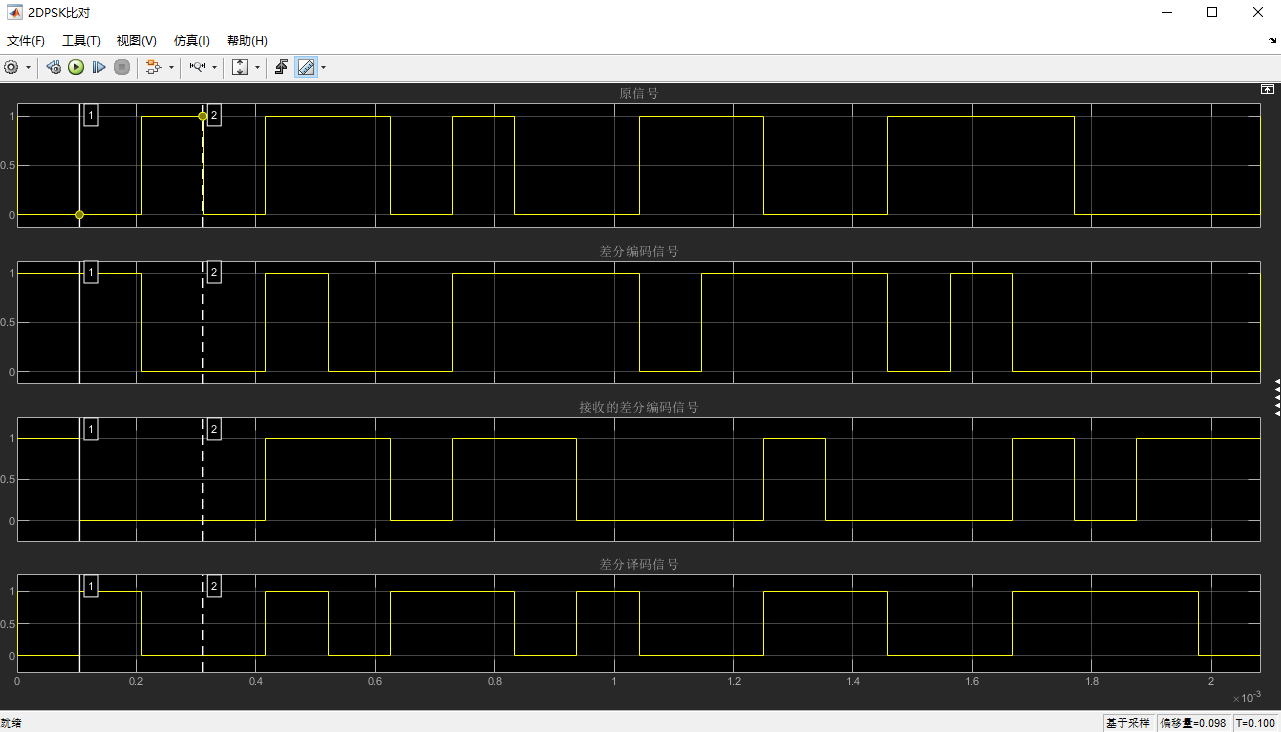
\includegraphics[width=5.9in]{texture/result/2dpsk比对.png}
    \caption{2DPSK比对}
    \label{2DPSK比对}
\end{figure}

\begin{figure}[H]
    \centering
    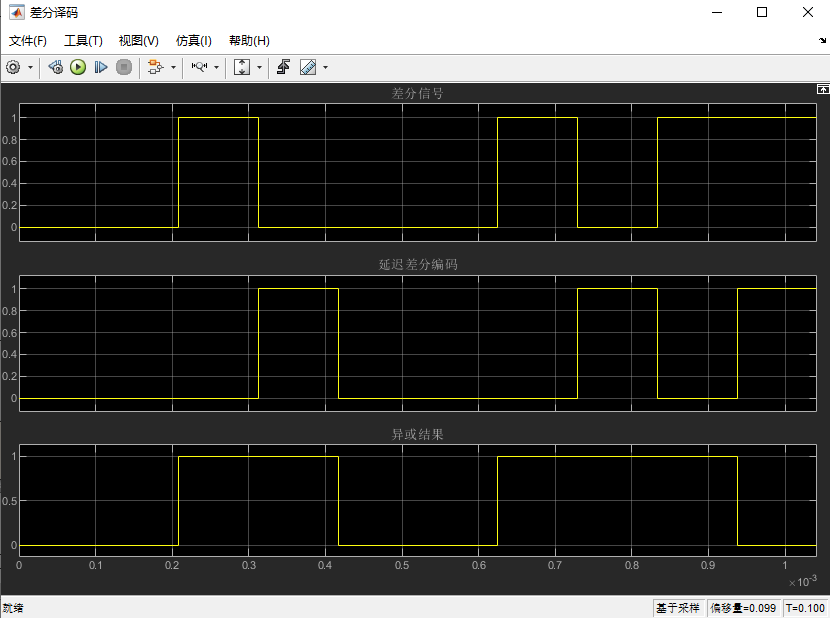
\includegraphics[width=5.9in]{texture/result/差分译码.png}
    \caption{差分译码}
    \label{差分译码}
\end{figure}

\subsection{相位模糊现象}

将接收方的载波信号反相后,发现2PSK的误码率接近100\%,而2DPSK不受影响。

因为载波信号反相会导致抽样判决后的信号全部翻转,1变0、0变1。但是2DPSK在抽样判决后是差分信号,需要再
进行差分译码才是结果;而差分信号是否翻转完全不影响差分译码的结果。

\subsection{误码曲线}

将高斯白噪声通道设为Eb/No模式并将Eb/No(dB)属性设为EbNo。
然后使用bertool工具读取输出到工作区的误码信息来绘制图像,并与理论值对比。

曲线见图\ref{误码曲线}。可见2PSK比2DPSK的抗噪声性能更好。

\begin{figure}[H]
    \centering
    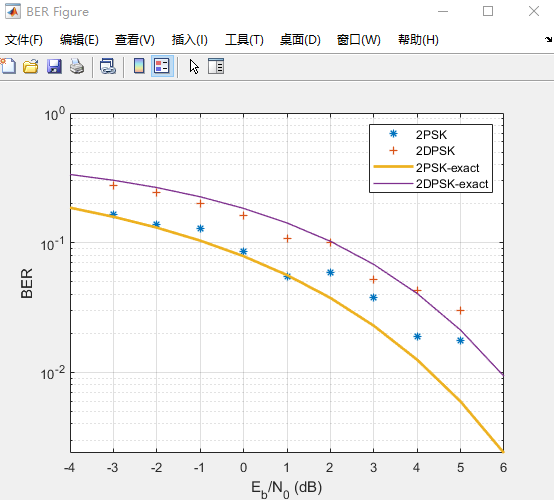
\includegraphics[width=5in]{texture/result/误码曲线.png}
    \caption{误码曲线}
    \label{误码曲线}
\end{figure}

\section{心得}

在2DPSK调制解调中,差分编码译码涉及到了逻辑操作,此时输出是bool类型,在显示与功能上都有可能出问题。
因此,我们要求每个涉及到bool的组件最后都必须输出double类型(使用Data Type Conversion组件)。

滤波器的延迟是我们之前未考虑到的东西。后来才发现延迟与阶数有关,而默认阶数与Fs有关。经过多次测试检验,
发现现在的参数是最佳的,即使使用默认的阶数也能很好地采样、解调。

此外,我们也更加熟悉了多个MATLAB Simulink组件,也学会了bertool的使用,
同时加深了对滤波器、采样、信号运算等理论知识的理解。

\end{document}

